\documentclass[tikz,border=4pt]{standalone}
\usepackage{amsmath}
\usepackage{tikz-cd}
\begin{document}
% CommGroup as a full subcategory of Group: a nested-box containment
% diagram, not a commutative square, so plain tikz rather than tikz-cd.
% Source: 01-basics/04-terminology.md, "subobject" glossary entry.
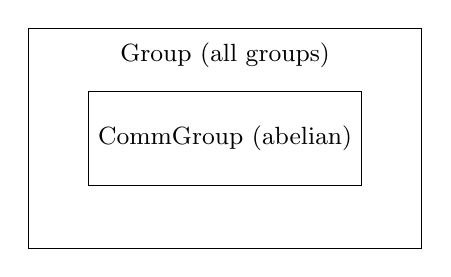
\begin{tikzpicture}[every node/.style={font=\small}]
  \node[draw, minimum width=5cm, minimum height=2.8cm] (outer) {};
  \node[anchor=north, yshift=-2pt] at (outer.north) {$\mathrm{Group}$ (all groups)};
  \node[draw, minimum width=3cm, minimum height=1.2cm] (inner) at (outer.center) {$\mathrm{CommGroup}$ (abelian)};
\end{tikzpicture}
\end{document}
